%----------------------------------------------------------------------------
%----------------------------------------------------------------------------
%----------------------------------------------------------------------------
%bb defines the bounding box for the pdf
%viewport defines the area of the pdf used
%in sidewaysfigure the last entry in bb moves the caption toward/away the pic
%in sidewaysfigure the second entry in bb moves the pic toward/away the caption
%----------------------------------------------------------------------------
\begin{figure}
\scalebox{0.8}[0.8]{
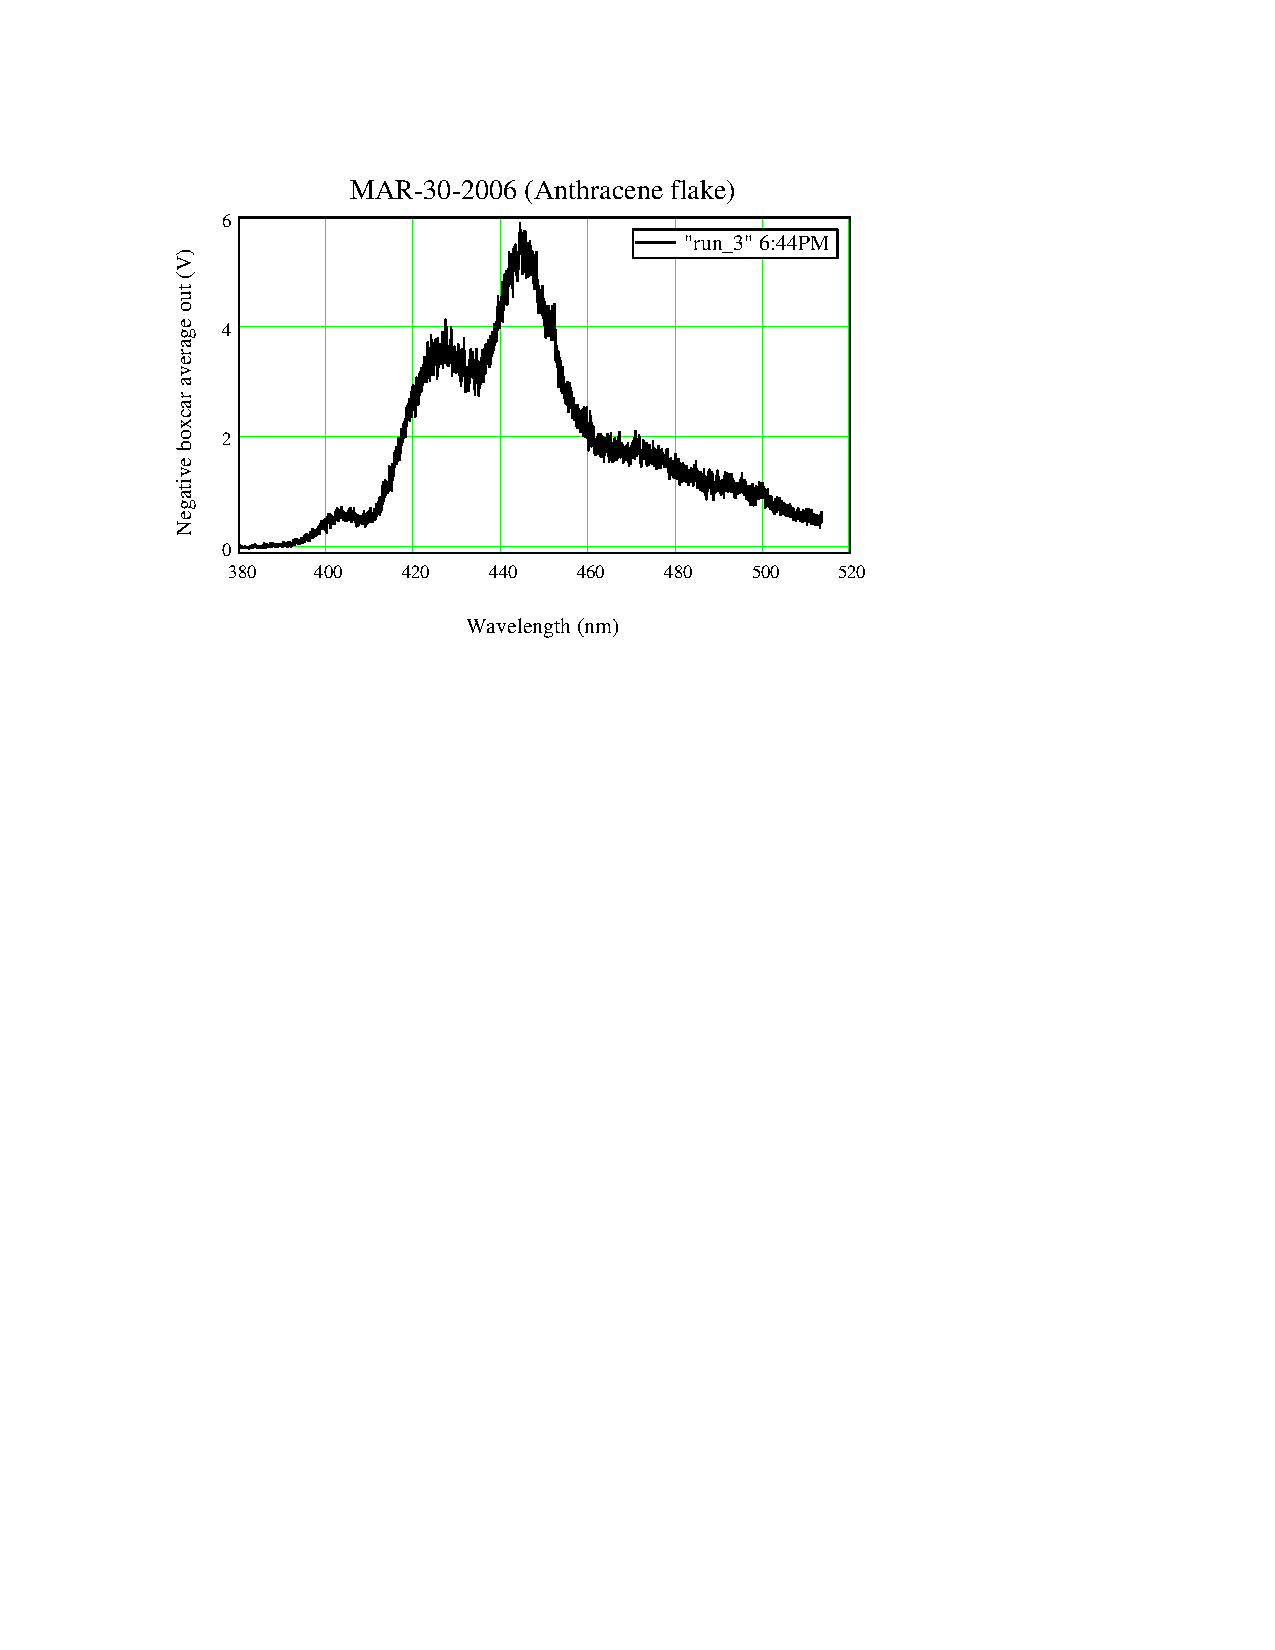
\includegraphics[bb=0 500 489 700]
{355_anthracene/355_anthracene.pdf}
}
\caption[LIF from a solid anthracene flake illuminated by a 355 nm YAG]{LIF from a solid anthracene flake illuminated by a 355 nm YAG}
\label{355_anthracene}
\end{figure}
%----------------------------------------------------------------------------

%----------------------------------------------------------------------------
%bb defines the bounding box for the pdf
%viewport defines the area of the pdf used
%in sidewaysfigure the last entry in bb moves the caption toward/away the pic
%in sidewaysfigure the second entry in bb moves the pic toward/away the caption
%----------------------------------------------------------------------------
\begin{figure}
\scalebox{0.8}[0.8]{
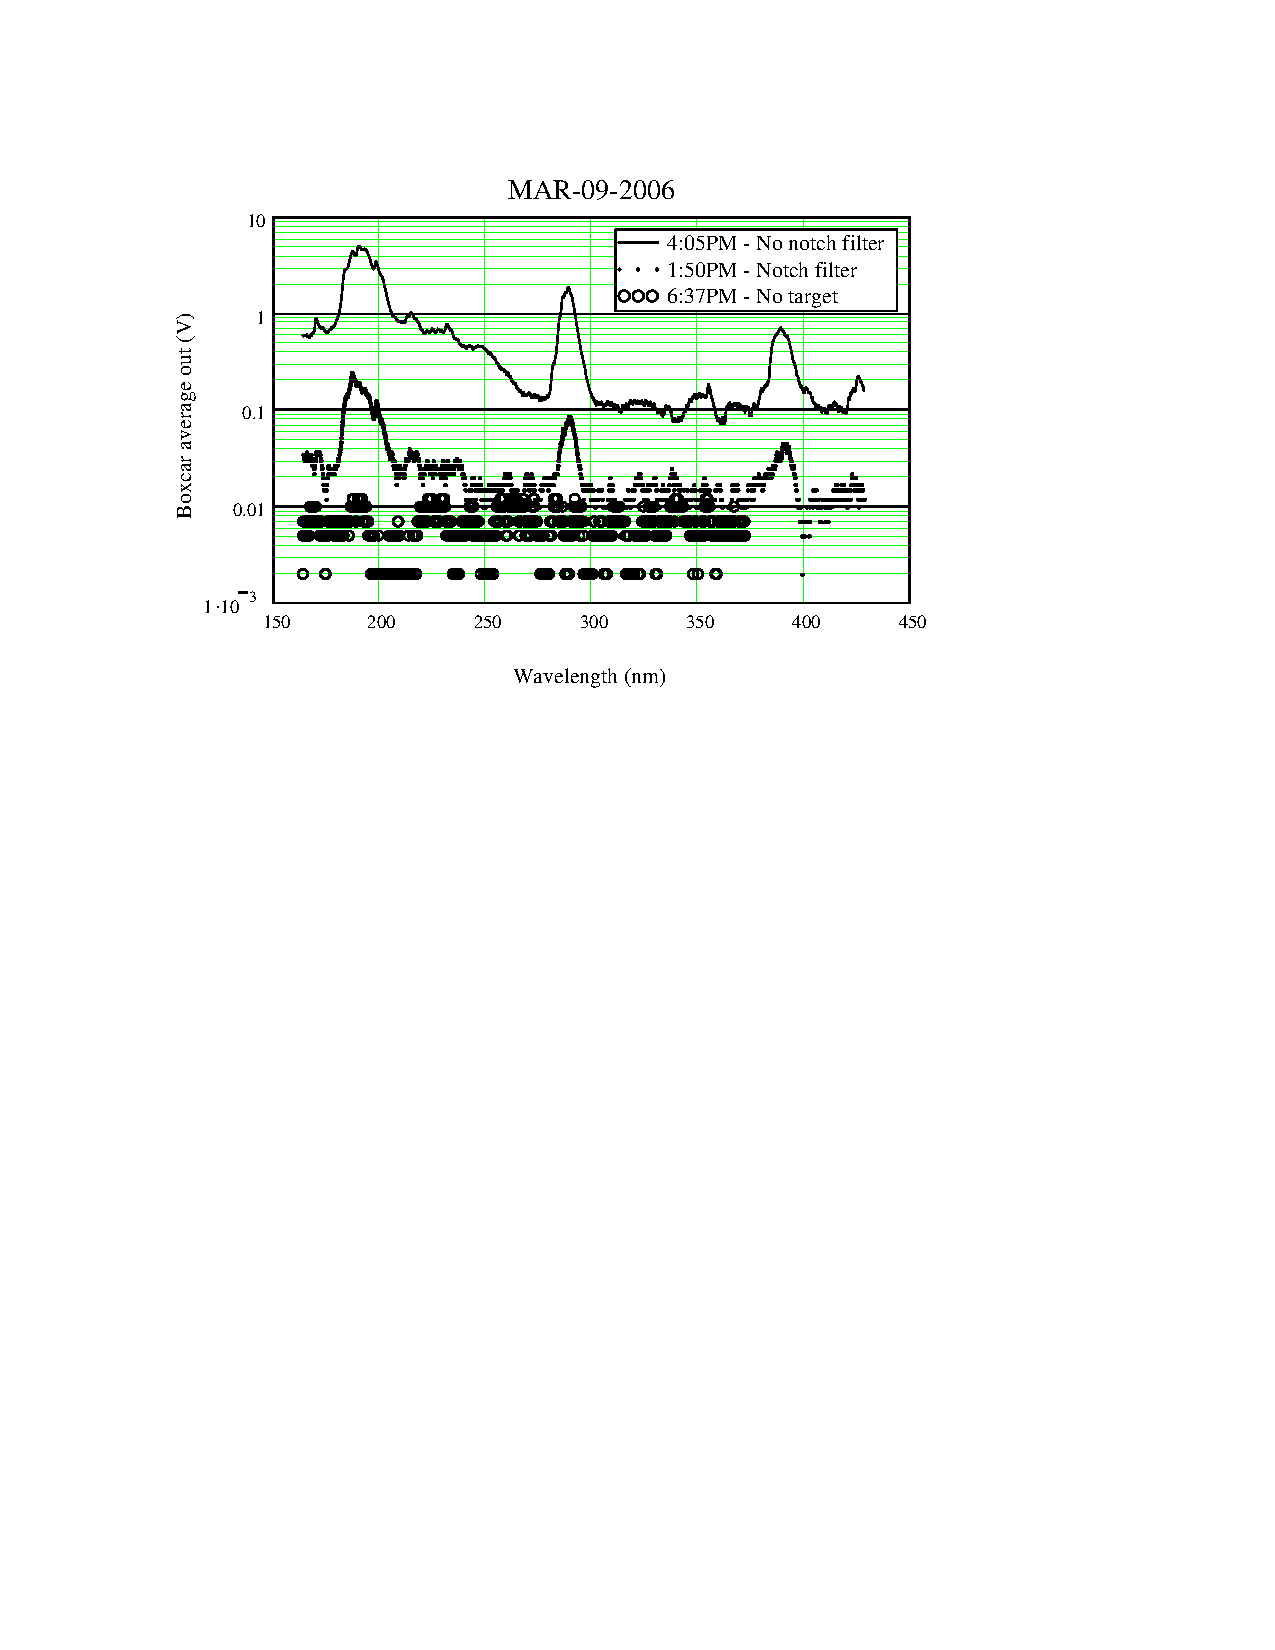
\includegraphics[bb=0 470 489 700]
{1064_ghosts/1064_ghosts.pdf}
}
\caption[Grating ghosts from 1064 nm laser illumination]{Grating ghosts from 1064 nm laser illumination. Using various targets (aromatic compounds, paper, and a calibrated Lambertian target) it was discovered that the spectral ``features'' observed in the UV were independent of the target. Then from the data shown here, acquired using a notch filter made for 1064 nm YAG output, it was concluded that the ``features'' were linearly related in intensity to the 1064 nm excitation and thus most likely ``ghost lines'' associated with the grating.}
\label{1064_ghosts}
\end{figure}
%----------------------------------------------------------------------------

%----------------------------------------------------------------------------
Measurements of the fluorescence response of aromatic compounds to YAG illumination have revealed some shortcomings of the 1 m monochromator. Figure \ref{355_anthracene} shows the LIF from an solid anthracene sample when excited by the output of a tripled Nd:YAG laser (355 nm). When the excitation is shifted to the doubled or fundamental output of the YAG, a complicated faint spectrum emerges in the scans. It was discovered that the faint features were independent of the target (paper and a white Lambertian target generated the same features). See Figure \ref{1064_ghosts} for the ghost lines resulting from fundamental YAG (1.06 um) illumination. It is believed that these are ``ghost lines'' from sub-periods in the groove spacing \cite{Palmer:2002a}. A holographic replacement grating (which should be free of ghost lines) is being procured.
%----------------------------------------------------------------------------
%----------------------------------------------------------------------------
%----------------------------------------------------------------------------
%----------------------------------------------------------------------------
%----------------------------------------------------------------------------
%----------------------------------------------------------------------------
